% Plain-language project report.
% Build:  cd project_report && tectonic project_report.tex   (or latexmk -xelatex project_report.tex)
\documentclass[10pt,a4paper]{article}

\usepackage[a4paper,margin=17mm,bottom=18mm]{geometry}
\usepackage{fontspec}
\setmainfont{texgyreheros}[Extension=.otf, UprightFont=*-regular, BoldFont=*-bold,
  ItalicFont=*-italic, BoldItalicFont=*-bolditalic]
\setmonofont{texgyrecursor}[Extension=.otf, UprightFont=*-regular, BoldFont=*-bold, Scale=0.95]
\usepackage{xcolor}
\usepackage{graphicx}
\usepackage{tabularx}
\usepackage{booktabs}
\usepackage{colortbl}
\usepackage{enumitem}
\usepackage{ragged2e}
\usepackage{fancyhdr}
\usepackage{tikz}
\usetikzlibrary{arrows.meta,positioning}
\usepackage[most]{tcolorbox}
\usepackage[hidelinks]{hyperref}

\graphicspath{{../results/figures/}{../app/screenshots/}}

% ---------------------------------------------------------------- palette
\definecolor{ink}{HTML}{111110}
\definecolor{ink2}{HTML}{4A4945}
\definecolor{muted}{HTML}{8A8882}
\definecolor{rulec}{HTML}{E4E3DD}
\definecolor{panel}{HTML}{F6F5F1}
\definecolor{accent}{HTML}{2A78D6}
\definecolor{accentsoft}{HTML}{EAF2FC}
\definecolor{notefg}{HTML}{24456E}
\definecolor{barlight}{HTML}{A9C8EE}
\definecolor{sgreen}{HTML}{0CA30C}
\definecolor{samber}{HTML}{EDA100}
\definecolor{sorange}{HTML}{EC835A}
\definecolor{sred}{HTML}{D03B3B}

% ---------------------------------------------------------------- page style
\pagestyle{fancy}
\fancyhf{}
\renewcommand{\headrulewidth}{0pt}
\fancyfoot[R]{\color{muted}\footnotesize\thepage}
\setlength{\parindent}{0pt}
\setlength{\parskip}{2.2mm}
\linespread{1.12}
\color{ink2}
\AtBeginDocument{\RaggedRight}
\setlist{leftmargin=4.5mm, itemsep=0.8mm, topsep=0.5mm, parsep=0pt, label={\color{ink2}\textbullet}}
\arrayrulecolor{rulec}
\setlength{\fboxsep}{0pt}
\setlength{\fboxrule}{0.4pt}

% ---------------------------------------------------------------- building blocks
\newcommand{\eyebrow}[1]{{\color{accent}\scriptsize\bfseries\addfontfeature{LetterSpace=14}\MakeUppercase{#1}}\par\vspace{-1mm}}
\newcommand{\pagetitle}[1]{{\color{ink}\fontsize{17}{21}\selectfont\bfseries #1}\par\vspace{1mm}}
\newcommand{\subhead}[1]{\vspace{1.5mm}{\color{ink}\bfseries #1}\par\vspace{-1mm}}
\newcommand{\lead}[1]{{\fontsize{10.6}{15.5}\selectfont #1}\par}
\newcommand{\bold}[1]{{\color{ink}\bfseries #1}}
\newcommand{\figcap}[2]{\par\vspace{1.2mm}{\color{muted}\footnotesize\linespread{1.05}\selectfont{\color{ink2}\bfseries #1} #2}\par}
\newcommand{\shot}[2][\dimexpr\linewidth-0.8pt\relax]{\fcolorbox{rulec}{white}{\includegraphics[width=#1]{#2}}}
\newcommand{\code}[1]{{\color{ink}\ttfamily\small #1}}
\newcommand{\dotc}[1]{\tikz[baseline=-0.6ex]\fill[#1] (0,0) circle (1.1mm);\,}

\newtcolorbox{stat}{enhanced, colback=panel, boxrule=0pt, frame hidden, arc=2.5mm,
  left=3mm, right=3mm, top=2.5mm, bottom=2.5mm}
\newcommand{\statbox}[2]{\begin{stat}{\color{ink}\fontsize{16}{18}\selectfont\bfseries #1}\par\vspace{0.6mm}
  {\scriptsize\linespread{1}\selectfont #2}\end{stat}}

\newtcolorbox{card}[1][]{enhanced, colback=white, colframe=rulec, boxrule=0.4pt, arc=2.5mm,
  left=3mm, right=3mm, top=2.5mm, bottom=2.5mm, before upper={\setlength{\parskip}{1mm}\small}, #1}
\newcommand{\cardtag}[1]{{\color{muted}\tiny\bfseries\addfontfeature{LetterSpace=8}\MakeUppercase{#1}}\par}
\newcommand{\cardtitle}[1]{{\color{ink}\bfseries #1}\par}

\newtcolorbox{note}{enhanced, colback=accentsoft, boxrule=0pt, frame hidden, arc=2.5mm,
  left=3.5mm, right=3.5mm, top=2.5mm, bottom=2.5mm, fontupper=\small\color{notefg}}

\newtcolorbox{codebox}{enhanced, colback=panel, boxrule=0pt, frame hidden, arc=2.5mm,
  left=3.5mm, right=3.5mm, top=2mm, bottom=2mm, fontupper=\ttfamily\small\color{ink}}

% table header cell
\newcommand{\hcell}[1]{{\color{muted}\scriptsize\bfseries\addfontfeature{LetterSpace=6}\MakeUppercase{#1}}}
\newcolumntype{R}{>{\raggedleft\arraybackslash}X}
\newcolumntype{L}{>{\raggedright\arraybackslash}X}

% feature-ablation bar: {label}{fraction of track}{value}{fill colour}
\newcommand{\fbar}[4]{%
  \makebox[24mm][l]{\footnotesize #1}%
  \tikz[baseline=-0.7ex]{\fill[panel,rounded corners=0.8mm] (0,-1.9mm) rectangle (42mm,1.9mm);
    \fill[#4,rounded corners=0.8mm] (0,-1.9mm) rectangle (#2*42mm,1.9mm);}%
  \hfill{\color{ink}\footnotesize\bfseries #3}\par\vspace{0.4mm}}

\begin{document}

% ================================================================ COVER
\begin{titlepage}
\newgeometry{margin=22mm,top=28mm,bottom=18mm}
\color{ink2}
{\color{accent}\footnotesize\bfseries\addfontfeature{LetterSpace=16}APPLIED MACHINE LEARNING \textbullet{} PROJECT REPORT}\par
\vspace{5mm}
{\color{ink}\fontsize{30}{33}\selectfont\bfseries Predicting Los Angeles\\[1mm] freeway traffic, one hour ahead}\par
\vspace{5mm}
\begin{minipage}{140mm}\fontsize{12}{18}\selectfont
A machine-learning system that reads live speeds from 207 road sensors and forecasts how fast
traffic will be moving at each sensor over the next 60 minutes. The forecasts can be explored
in an interactive website.
\end{minipage}\par
\vspace{11mm}
\shot{live.jpg}
\vfill
{\color{rulec}\rule{\linewidth}{0.4pt}}\par\vspace{1mm}
{\footnotesize\color{muted}
\begin{tabularx}{\linewidth}{@{}LLL@{}}
{\color{ink}\bfseries Dataset} & {\color{ink}\bfseries Best model} & {\color{ink}\bfseries Website}\\
METR-LA \textperiodcentered{} 207 sensors \textperiodcentered{} Mar--Jun 2012 &
Graph WaveNet (graph neural network) & Streamlit app \textperiodcentered{} \code{app/app.py}
\end{tabularx}}
\restoregeometry
\end{titlepage}

% ================================================================ 1 AT A GLANCE
\eyebrow{01 \textperiodcentered{} At a glance}
\pagetitle{What this project does, in one page}
\lead{Navigation apps, traffic control rooms and emergency services all need to know what traffic
will look like \emph{soon}, not just right now. This project builds and compares several
machine-learning models that look at the last hour of traffic on Los Angeles freeways and predict
the speed at every sensor for each of the next twelve 5-minute steps (5 to 60 minutes ahead).}

\begin{tcbraster}[raster columns=4, raster equal height, raster column skip=3mm]
\statbox{3.07 {\normalsize\mdseries mph}}{Average forecast error of the best model, across all 12 steps}
\statbox{2.72 {\normalsize\mdseries mph}}{Error 15 minutes ahead. Traffic is easier to predict in the short term}
\statbox{27\%}{Less error than the simple ``usual speed for this time'' guess}
\statbox{207}{Sensors forecast at once, every 5 minutes}
\end{tcbraster}

\subhead{The journey, step by step}
\begin{center}
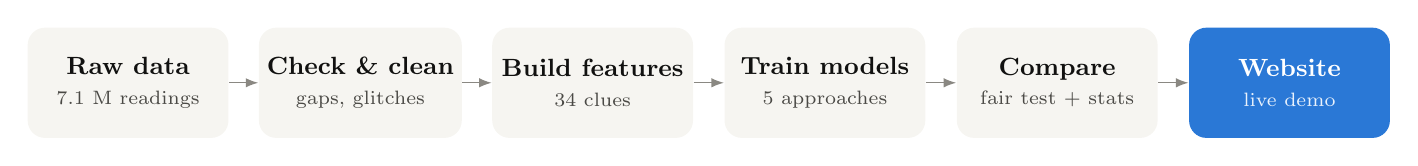
\begin{tikzpicture}[
  box/.style={rounded corners=2.2mm, fill=panel, minimum width=25.5mm, minimum height=14mm, align=center, inner sep=1mm},
  arr/.style={-{Latex[length=1.6mm]}, draw=muted, line width=0.5pt}]
  \foreach \i/\t/\s in {0/Raw data/7.1 M readings, 1/Check \& clean/{gaps, glitches},
                        2/Build features/34 clues, 3/Train models/5 approaches, 4/Compare/fair test + stats}
    \node[box] (b\i) at (\i*29.5mm,0) {{\color{ink}\small\bfseries \t}\\[-0.5mm]{\scriptsize\color{ink2}\s}};
  \node[box, fill=accent] (b5) at (5*29.5mm,0) {{\color{white}\small\bfseries Website}\\[-0.5mm]{\scriptsize\color{accentsoft}live demo}};
  \foreach \i [evaluate=\i as \j using int(\i+1)] in {0,...,4} \draw[arr] (b\i) -- (b\j);
\end{tikzpicture}
\end{center}

\begin{minipage}[t]{0.48\linewidth}
\subhead{The question}
Given the speed at all 207 sensors over the \bold{last 60 minutes}, and a map of how the sensors
are connected by road, what will the speed be at each sensor \bold{5, 10, \ldots{} 60 minutes from now}?

\subhead{Why it is hard}
\begin{itemize}
  \item \bold{Sudden jams.} Speed can drop from 65 to 20 mph within minutes.
  \item \bold{Rush hours.} Traffic follows daily and weekly rhythms.
  \item \bold{Jams spread.} A slowdown at one point moves backwards up the road to other sensors.
  \item \bold{Broken sensors.} About 8\% of readings are missing.
\end{itemize}
\end{minipage}\hfill
\begin{minipage}[t]{0.48\linewidth}
\subhead{What we found}
\begin{itemize}
  \item A \bold{graph neural network} (Graph WaveNet), which learns how sensors influence each
        other, was the most accurate model at every horizon.
  \item A much simpler \bold{gradient boosting} model with well-designed inputs came close: only
        0.07 mph behind at 60 minutes.
  \item Statistical tests confirm the best model's lead is real, not luck (\emph{p}\,<\,0.001).
  \item Our result is within 0.03--0.06 mph of the published Graph WaveNet paper, so the
        implementation is faithful.
  \item All of it can be explored in a \bold{web app} that replays any moment of the test period.
\end{itemize}
\end{minipage}

\newpage
% ================================================================ 2 DATA
\eyebrow{02 \textperiodcentered{} The data}
\pagetitle{207 sensors, four months, every five minutes}
\lead{We use \bold{METR-LA}, the standard public benchmark for traffic forecasting. Loop detectors
buried in the road on Los Angeles County freeways record the average vehicle speed every 5 minutes.
Because so many research papers use it, our numbers can be compared directly with published work.}

\begin{minipage}[t]{0.45\linewidth}\vspace{0pt}
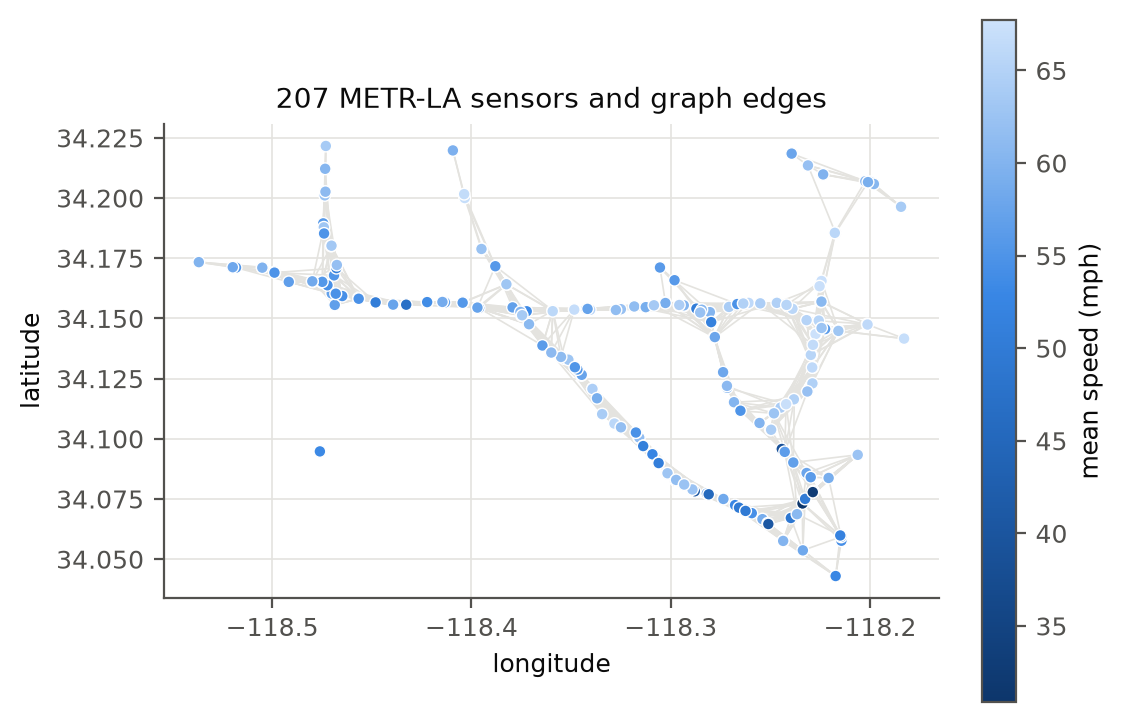
\includegraphics[width=\linewidth]{eda_sensor_map.png}
\figcap{Where the sensors are.}{Each dot is a sensor, coloured by its average speed (darker is slower).
The grey lines join sensors that are close along the road. These links form the ``graph'' the best model uses.}
\end{minipage}\hfill
\begin{minipage}[t]{0.51\linewidth}\vspace{0pt}
\small
\begin{tabularx}{\linewidth}{@{}Lr@{}}
\hcell{Property} & \hcell{Value}\\ \midrule
Sensors & 207\\ \midrule
Period & 1 Mar -- 27 Jun 2012\\ \midrule
Readings per sensor & 34,272 (119 days)\\ \midrule
Total readings & 7.09 million\\ \midrule
Average speed & 58.5 mph\\ \midrule
Speed limit of the sensors & capped at 70 mph\\ \midrule
Readings under 40 mph (jams) & 10.9\%\\ \midrule
Missing readings & 8.1\%\\ \midrule
Road links between sensors & 1,515\\ \midrule
\end{tabularx}
\par\vspace{1mm}
The data also comes with the GPS location of each sensor and the driving distance between pairs of
sensors. We use those distances to build the road map.
\end{minipage}

\subhead{What exploring the data told us}
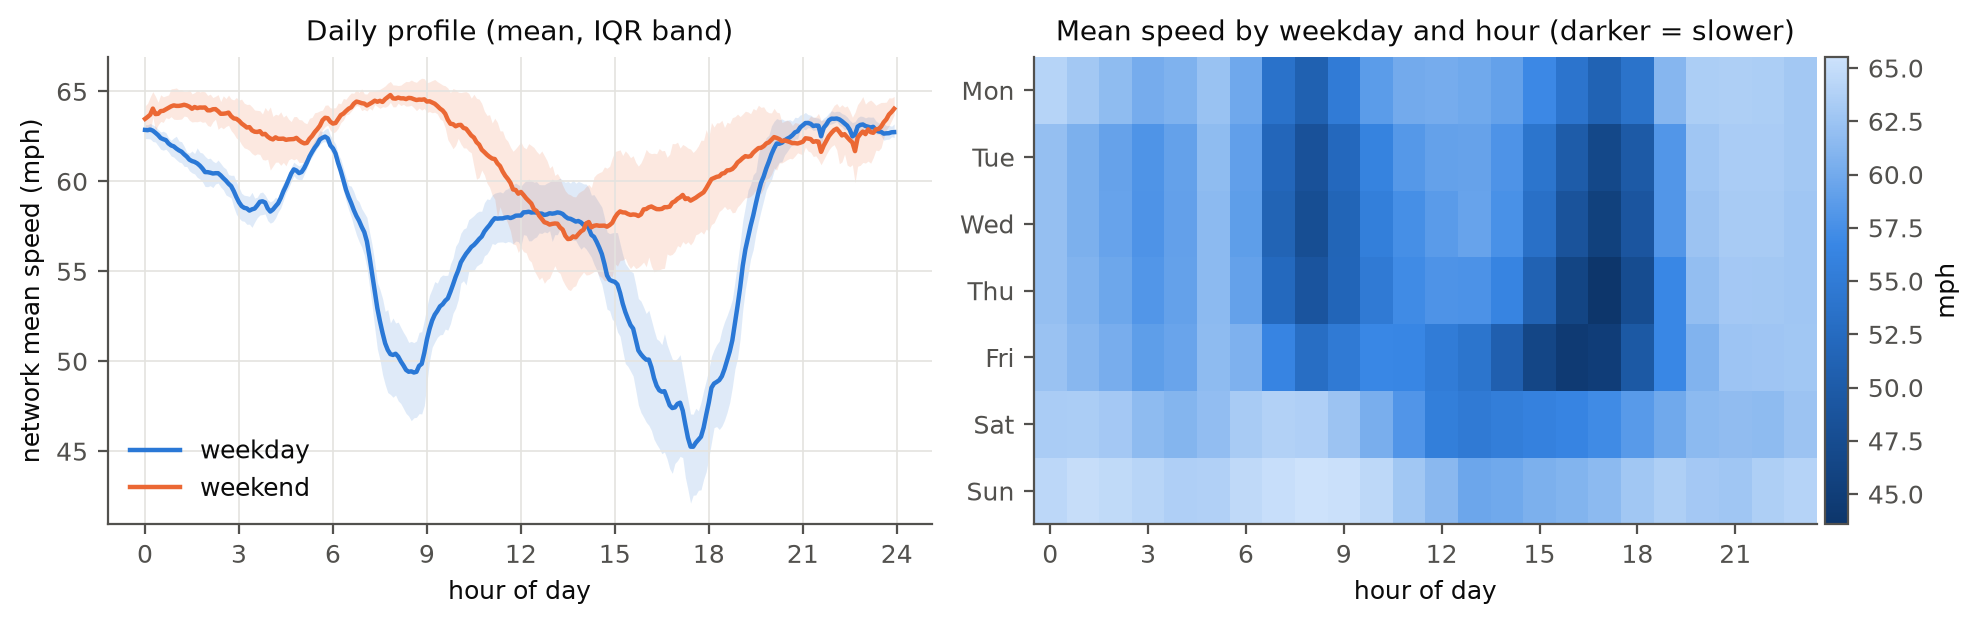
\includegraphics[width=\linewidth]{eda_daily_profile.png}
\figcap{The rhythm of the week.}{Left: average network speed across the day. Weekdays (blue) have a
clear morning dip around 8:30 and a deeper evening dip around 17:30; weekends (orange) stay fast.
Right: the same pattern by day of the week. Darker cells are slower, so Tuesday--Friday evenings are the worst.}
\vspace{2mm}

\begin{tcbraster}[raster columns=3, raster equal height, raster column skip=3mm]
\begin{card}\cardtag{Finding}\cardtitle{Strong weekly rhythm}Each sensor's ``usual speed for this time of
the week'' is a powerful clue, so we turned it into a feature.\end{card}
\begin{card}\cardtag{Finding}\cardtitle{Recent past matters most}Speed 5 minutes ago is 86\% correlated
with speed now, but that link fades fast. Long-range forecasts need more than the last reading.\end{card}
\begin{card}\cardtag{Finding}\cardtitle{Neighbours move together}Sensors joined by road are about
4× more correlated in their unusual swings than unconnected ones. This is why a road-map-aware
model helps.\end{card}
\end{tcbraster}

\newpage
% ================================================================ 3 CLEANING
\eyebrow{03 \textperiodcentered{} Data quality}
\pagetitle{Checking and cleaning the readings}
\lead{Real sensors fail. Before modelling, every reading went through a set of automatic checks.
Missing values show up in the file as \bold{0 mph}, which is easy to mistake for a total
standstill, so they have to be found and handled carefully.}

\begin{minipage}[t]{0.48\linewidth}
\subhead{What was checked}
\begin{itemize}
  \item \bold{12 integrity checks}: timestamps exactly 5 minutes apart, no duplicate sensors,
        every speed between 0 and 70 mph, every sensor inside Los Angeles, and so on. All 12 passed.
  \item \bold{Network outages}: moments when \emph{all} 207 sensors read 0 at once (2,148 time
        steps, 6.3\% of data).
  \item \bold{Single sensor missing}: one sensor reads 0 while its neighbours are fine (1.8\%).
  \item \bold{Spikes}: a one-off jump far from the surrounding readings (6,142 readings).
  \item \bold{Stuck sensors}: the same value repeated for over an hour (274 readings).
\end{itemize}
\end{minipage}\hfill
\begin{minipage}[t]{0.48\linewidth}
\subhead{How gaps were filled}
We hid random stretches of good data, filled them in with several methods, and measured which guessed best:
\begin{itemize}
  \item \bold{Short gaps (up to 1 hour):} draw a straight line between the readings on either side.
  \item \bold{Long gaps:} use the sensor's usual speed for that time of the week. For a 24-hour gap
        this was twice as accurate (4.0 vs 8.6 mph error).
\end{itemize}
\vspace{1mm}
\begin{note}\textbf{Important detail.} Good readings are never changed. And the models are still
\textbf{scored only on real readings}, never on filled-in ones, so that our results stay comparable
with published research.\end{note}
\end{minipage}

\vspace{3mm}
\begin{center}
\begin{minipage}{0.88\linewidth}
\shot{quality.jpg}
\figcap{Website, ``Data quality'' tab.}{One sensor on one day: raw readings (grey), the cleaned series
(blue) and flagged readings (orange crosses).}
\vspace{2mm}
\shot{quality2.jpg}
\figcap{Lower half of the same tab.}{Left: share of readings flagged, by type. Network outages dominate.
Right: error of each gap-filling method as gaps get longer. Our hybrid rule (blue) stays lowest
across all gap lengths.}
\end{minipage}
\end{center}

\newpage
% ================================================================ 4 MODELS
\eyebrow{04 \textperiodcentered{} The models}
\pagetitle{Five ways to forecast, from simple to smart}
\lead{To know whether a complex model is worth it, you need simple ones to beat. We built a
``ladder'' of five forecasters. Every model sees exactly the same data and is scored the same way.}

\begin{tcbraster}[raster columns=2, raster equal height=rows, raster column skip=3.5mm, raster row skip=3mm]
\begin{card}\cardtag{Baseline}\cardtitle{1 \textperiodcentered{} Historical Average}``Traffic will be at its
usual speed for this time on this weekday.'' Ignores what is happening right now.\end{card}
\begin{card}\cardtag{Baseline}\cardtitle{2 \textperiodcentered{} Persistence}``Speed will stay exactly as it
is now.'' Hard to beat 5 minutes ahead, poor an hour ahead.\end{card}
\begin{card}\cardtag{Classical ML}\cardtitle{3 \textperiodcentered{} Ridge regression}A weighted sum of 34
hand-made clues (features). Fast and easy to explain, but can only learn straight-line relationships.\end{card}
\begin{card}\cardtag{Classical ML}\cardtitle{4 \textperiodcentered{} Gradient Boosting}Hundreds of small
decision trees, each fixing the previous ones' mistakes. Uses the same 34 clues but can learn curved,
``if-this-then-that'' patterns.\end{card}
\end{tcbraster}
\vspace{1mm}
\begin{card}[colback=accentsoft, colframe=accent]
{\color{accent}\tiny\bfseries\addfontfeature{LetterSpace=8}DEEP LEARNING \textbullet{} BEST MODEL}\par
\cardtitle{5 \textperiodcentered{} Graph WaveNet}
{\color{notefg}A graph neural network. It treats the sensors as points on a network and learns how
traffic at one sensor affects others. It uses the real road map, plus a second, \textbf{self-learned
map} that can find links the roads alone don't show. Over time, it uses stacked convolution layers
that look back at different time scales. It has about 301,000 learnable numbers and took 2.4 hours
to train on a laptop (Apple M3).}
\end{card}

\subhead{The 34 clues given to the classical models}
Deep models discover patterns by themselves; classical models need them spelled out. We built six
groups of features. Every one uses \bold{only past information}, and automated tests check that no
future data leaks in.
\vspace{1mm}

\begin{minipage}[t]{0.53\linewidth}\vspace{0pt}
\small
\renewcommand{\arraystretch}{1.15}
\begin{tabularx}{\linewidth}{@{}>{\color{ink}\bfseries}p{24mm}L@{}}
\hcell{Group} & \hcell{Plain-language meaning}\\ \midrule
Lags & Speed now, 5 min ago, 10 min ago \ldots{} up to an hour ago\\ \midrule
Window stats & Average, spread and minimum over the last hour; how many readings were missing\\ \midrule
Calendar & Time of day and day of week of the moment being predicted\\ \midrule
Weekly profile & This sensor's usual speed at this time of week, and how far today differs from usual\\ \midrule
Spatial & Average speed of the sensors just upstream and just downstream on the road\\ \midrule
Sensor & Fixed facts about the sensor, such as its overall average and how connected it is\\ \midrule
\end{tabularx}
\end{minipage}\hfill
\begin{minipage}[t]{0.43\linewidth}\vspace{0pt}
{\color{ink}\bfseries How much each group helped}\par\vspace{0.5mm}
{\footnotesize Gradient Boosting, 60 min ahead. Groups were added one at a time; bars show the error
(mph) after each addition. Shorter is better.}\par\vspace{2mm}
\fbar{Lags only}{1.000}{4.36}{barlight}
\fbar{+ window stats}{0.996}{4.34}{barlight}
\fbar{+ calendar}{0.909}{3.96}{barlight}
\fbar{+ weekly profile}{0.807}{3.52}{accent}
\fbar{+ spatial}{0.787}{3.43}{barlight}
\fbar{+ sensor}{0.782}{3.41}{barlight}
\vspace{1.5mm}
{\footnotesize Knowing \bold{``what is normal for this sensor at this time''} was the single most
valuable clue. Altogether the features cut the 60-minute error by 22\%.}
\end{minipage}

\newpage
% ================================================================ 5 RESULTS
\eyebrow{05 \textperiodcentered{} Results}
\pagetitle{Which model forecasts best?}
\lead{The models were trained on the first 70\% of the timeline (March to May), tuned on the next
10\%, and tested on the \bold{last 20\%} (4--27 June), which they had never seen. Splitting by time
like this mimics real use: you always predict the future from the past.}

\vspace{1mm}
{\small\renewcommand{\arraystretch}{1.25}
\begin{tabularx}{\linewidth}{@{}LRRRR@{}}
\hcell{Model} & \hcell{15 min} & \hcell{30 min} & \hcell{60 min} & \hcell{Average}\\ \midrule
\rowcolor{accentsoft}{\color{ink}\bfseries Graph WaveNet} & {\color{ink}\bfseries 2.72} & {\color{ink}\bfseries 3.10} & {\color{ink}\bfseries 3.59} & {\color{ink}\bfseries 3.07}\\ \midrule
Gradient Boosting & 2.89 & 3.29 & 3.66 & 3.22\\ \midrule
Ridge regression & 3.37 & 3.78 & 4.09 & 3.69\\ \midrule
Persistence & 3.50 & 4.21 & 5.38 & 4.24\\ \midrule
Historical Average & 4.19 & 4.19 & 4.19 & 4.19\\ \midrule
\end{tabularx}}
{\color{muted}\footnotesize Mean absolute error (MAE) in mph: on average, how far the forecast was from
the real speed. Lower is better. Missing readings are ignored.}

\vspace{3mm}
\shot{accuracy.jpg}
\figcap{Website, ``Model accuracy'' tab.}{Error rises the further ahead we predict. Persistence (yellow)
gets worse fastest, Historical Average (pink) stays flat, and Graph WaveNet (blue) is lowest at every
horizon. The chart can be switched between MAE, RMSE and MAPE, and the tab also lists the full table above.}
\vspace{2mm}

\begin{minipage}[t]{0.48\linewidth}
\subhead{Is the win real?}
Small differences can be luck. We used the \bold{Diebold--Mariano test}, a standard way to compare
two forecasters, and \bold{bootstrap confidence intervals}, which resample whole days to see how
stable each score is. Graph WaveNet beats every other model at every horizon with \bold{\emph{p}\,<\,0.001}.
\end{minipage}\hfill
\begin{minipage}[t]{0.48\linewidth}
\subhead{How does it compare to research?}
The original Graph WaveNet paper reports 3.53 mph at 60 minutes; ours reaches 3.59. The well-known
DCRNN model reports 3.60, so \bold{our model matches published state-of-the-art results} under the
same test protocol.
\end{minipage}

\newpage
% ================================================================ 6 WEBSITE
\eyebrow{06 \textperiodcentered{} The website}
\pagetitle{An interactive forecast dashboard}
\lead{The trained Graph WaveNet model powers a web app built with \bold{Streamlit}. You pick any
moment in the test period, and the app runs the model on the hour of data before it, then shows the
forecast next to what really happened.}

\vspace{1mm}
\shot{live.jpg}
\figcap{``Live forecast'' tab, Monday 4 June 2012, 16:30.}{The top cards show the speed now and the
forecasts for +15, +30 and +60 minutes at the chosen sensor. The chart compares the forecast (blue)
with what was really measured (grey). The map colours every sensor by its predicted speed in 60
minutes. Here 93 of 207 sensors are expected to drop below 40 mph as the evening rush builds.}
\vspace{1mm}

\begin{minipage}[t]{0.48\linewidth}
\subhead{Controls (left sidebar)}
\begin{itemize}
  \item \bold{Date, time and sensor} pickers, then \emph{Run forecast}.
  \item \bold{Step through time} by 5 minutes or an hour, or \bold{jump} to morning, midday,
        evening or night.
  \item \bold{Play through the day} moves the clock forward automatically so you can watch jams form.
  \item \bold{Find a sensor}: the slowest right now, the one about to slow down most, the one with
        the biggest error, or a random one. You can also click any dot on the map.
\end{itemize}
\end{minipage}\hfill
\begin{minipage}[t]{0.48\linewidth}
\subhead{Four tabs}
\begin{itemize}
  \item \bold{Live forecast}: the next hour at one sensor plus the network map.
  \item \bold{Whole day}: every forecast for the day, made 15 or 60 minutes ahead.
  \item \bold{Model accuracy}: all five models compared on the full test set.
  \item \bold{Data quality}: cleaning results, flagged readings and the least reliable sensors.
\end{itemize}
\vspace{1mm}
{\footnotesize Map colours: \dotc{sgreen}free-flow ≥ 55 \textperiodcentered{}
\dotc{samber}slowing ≥ 40 \textperiodcentered{} \dotc{sorange}congested ≥ 25
\textperiodcentered{} \dotc{sred}severe < 25 mph.}
\end{minipage}

\newpage
% ================================================================ 7 LESSONS + CONCLUSION
\shot{day.jpg}
\figcap{``Whole day'' tab.}{Every forecast made 15 minutes ahead for a full day at one sensor (blue)
against what was really measured (grey). The model follows the evening slowdown closely. A second
chart below it (not shown) does the same for 60 minutes ahead, where the model still predicts the dip
but smooths out the sharpest drops.}
\vspace{4mm}

\eyebrow{07 \textperiodcentered{} Lessons and next steps}
\pagetitle{Where the model struggles, and what we learned}

\begin{minipage}[t]{0.45\linewidth}\vspace{0pt}
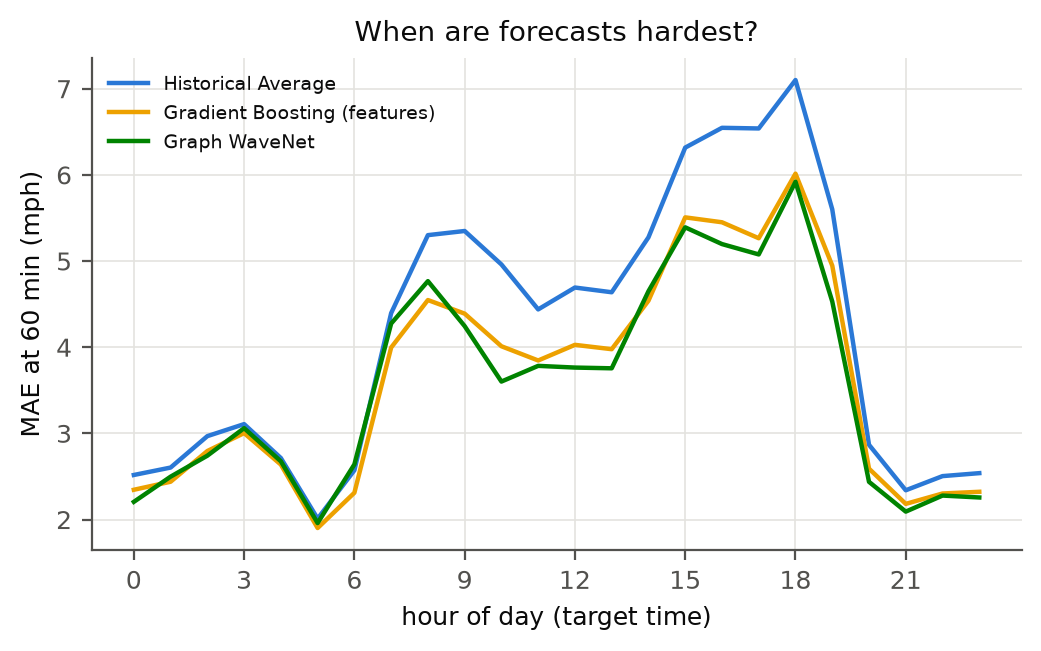
\includegraphics[width=\linewidth]{res_mae_by_hour.png}
\figcap{Error by time of day}{(60 min ahead). Night is easy; the evening rush around 18:00 is hardest
for every model.}
\end{minipage}\hfill
\begin{minipage}[t]{0.51\linewidth}\vspace{0pt}
\begin{itemize}
  \item \bold{Rush hour is hardest.} Errors peak near 6 mph around 18:00, about three times the
        night-time level, because jams start and clear suddenly.
  \item \bold{Missing inputs hurt the deep model more.} When a sensor's latest reading is missing,
        Graph WaveNet's 60-minute error rises to 5.36 mph, while Gradient Boosting rises only to
        4.50. The hand-made ``missing'' features help.
  \item \bold{Simple can be strong.} Gradient Boosting trains in about 10 minutes on a CPU and is
        nearly as good an hour ahead.
  \item \bold{Next steps:} add weather, incidents and events; train with simulated sensor
        failures; try newer Transformer-based models; serve live data instead of replaying 2012.
\end{itemize}
\end{minipage}

\subhead{Conclusion}
The project covers the full machine-learning pipeline: exploring and cleaning real sensor data,
designing leak-free features, training five models of increasing complexity, testing the results
statistically, and putting the best model in front of users. The graph neural network wins because
it learns how traffic flows between connected sensors. A well-designed classical model comes
surprisingly close.

\subhead{Run it yourself}
\begin{codebox}
\begin{tabular}{@{}l@{\hspace{8mm}}l@{}}
pip install -r requirements.txt \&\& pip install -e . & \\
pytest & {\color{muted}\# 32 automated tests}\\
streamlit run app/app.py & {\color{muted}\# open the website}
\end{tabular}
\end{codebox}
{\color{muted}\footnotesize Code: Python package in \code{src/traffic/}, one script per experiment in
\code{scripts/}, all results in \code{results/}. Key references: Li et al., \emph{DCRNN}, ICLR 2018;
Wu et al., \emph{Graph WaveNet}, IJCAI 2019.}

\end{document}
